% C.31 切线长定理: PA, PB 切线, ∠APB=60°, PA=4√3
\documentclass[tikz,border=4pt]{standalone}
\usepackage{ctex}
\usepackage{amsmath}
\usetikzlibrary{calc, arrows.meta}
\begin{document}
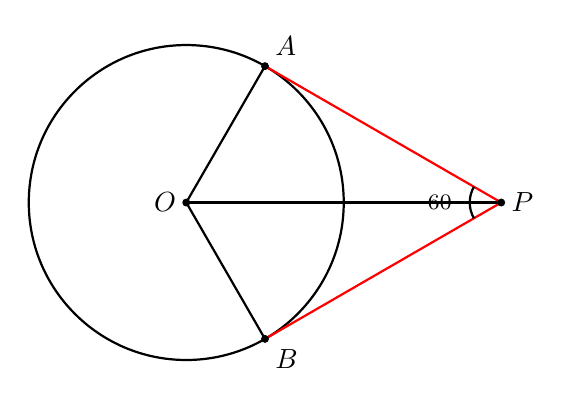
\begin{tikzpicture}[scale=0.5, thick]
  % PA=4√3≈6.93, ∠APO=30, so OA = PA tan30 = 4√3 * (√3/3)=4. OP=PA/cos30=4√3/(√3/2)=8.
  \coordinate (P) at (8,0);
  \coordinate (O) at (0,0);
  \draw (O) circle (4);
  \coordinate (A) at ({4*cos(60)}, {4*sin(60)});
  \coordinate (B) at ({4*cos(-60)}, {4*sin(-60)});
  \draw (O) -- (P);
  \draw (O) -- (A);
  \draw (O) -- (B);
  \draw[red] (P) -- (A);
  \draw[red] (P) -- (B);
  \filldraw (O) circle (2pt) node[left] {$O$};
  \filldraw (P) circle (2pt) node[right] {$P$};
  \filldraw (A) circle (2pt) node[above right] {$A$};
  \filldraw (B) circle (2pt) node[below right] {$B$};
  \draw ($(P)+(-0.8,0)$) arc (180:180-30:0.8);
  \draw ($(P)+(-0.8,0)$) arc (180:180+30:0.8);
  \node[font=\footnotesize, left] at ($(P)+(-1.0,0)$) {$60°$};
\end{tikzpicture}
\end{document}
